%%
%% Copyright 2007, 2008, 2009 Elsevier Ltd
%%
%% This file is part of the 'Elsarticle Bundle'.
%% ---------------------------------------------
%%
%% It may be distributed under the conditions of the LaTeX Project Public
%% License, either version 1.2 of this license or (at your option) any
%% later version.  The latest version of this license is in
%%    http://www.latex-project.org/lppl.txt
%% and version 1.2 or later is part of all distributions of LaTeX
%% version 1999/12/01 or later.
%%
%% The list of all files belonging to the 'Elsarticle Bundle' is
%% given in the file `manifest.txt'.
%%

%% Template article for Elsevier's document class `elsarticle'
%% with numbered style bibliographic references
%% SP 2008/03/01

\documentclass[preprint,12pt, a4paper]{elsarticle}

%% Use the option review to obtain double line spacing
%% \documentclass[authoryear,preprint,review,12pt]{elsarticle}

%% For including figures, graphicx.sty has been loaded in
%% elsarticle.cls. If you prefer to use the old commands
%% please give \usepackage{epsfig}

%% The amssymb package provides various useful mathematical symbols
\usepackage{amssymb}
%% The amsthm package provides extended theorem environments
%% \usepackage{amsthm}

%% The lineno packages adds line numbers. Start line numbering with
%% \begin{linenumbers}, end it with \end{linenumbers}. Or switch it on
%% for the whole article with \linenumbers.
\usepackage{lineno}

\usepackage{float}
\restylefloat{table}

% ======== additional package not in SoftwareX template ========
\usepackage[colorlinks=true, urlcolor=blue, pdfborder={0 0 0}]{hyperref}
\usepackage{breakurl}
\usepackage[htt]{hyphenat}
%\usepackage{listings}
%\usepackage{xcolor}
%\usepackage{todonotes}

% \let\oldtodo\todo
% \renewcommand{\todo}[1]{\oldtodo[tickmarkheight=0.5em]{#1}}

\newcommand{\comment}[1]{}
% =================================================

\journal{SoftwareX}

\begin{document}
\begin{frontmatter}

\title{\texttt{davos}: a Python package ``smuggler'' for constructing
  lightweight reproducible notebooks}
\author{Paxton C. Fitzpatrick}
\author{Jeremy R. Manning\corref{cor}}
\ead{Jeremy.R.Manning@Dartmouth.edu}
\cortext[cor]{Corresponding author}
\address{Department of Psychological and Brain Sciences\\Dartmouth College, Hanover, NH 03755}

% ------------------------------------------------------ ABSTRACT ------------------------------------------------------

\begin{abstract}
% 100-word limit (though many published articles don't seem to conform
% to this?)

  Reproducibility is a core requirement of modern scientific research.
  For computational research, reproducibility means that code should
  produce the same results, even when run on different systems.  A
  standard approach to ensuring reproducibility entails packaging a
  project's dependencies along with its primary code base.  Existing
  solutions vary in how deeply these dependencies are specified,
  ranging from virtual environments, to containers, to virtual
  machines.  Each of these existing solutions requires installing or
  setting up a system for running the desired code that must be
  packaged alongside the primary code base.  Here we propose a
  lighter-weight solution than virtual environments: the
  \texttt{davos} library.  When used in combination with a
  notebook-based Python project, the \texttt{davos} library provides a
  mechanism for specifying (and automatically installing) the correct
  package versions of the project's dependencies.  The \texttt{davos}
  library also ensures that those versions are in use any time the
  notebook's code is executed.  This enables researchers to share a complete
  reproducible environment using a single Jupyter notebook file.

\end{abstract}


\begin{keyword}
Reproducibility \sep Open science \sep Python \sep Jupyter Notebook \sep Google Colaboratory \sep Package management
\end{keyword}

\end{frontmatter}


% ------------------------------------------------------ METADATA ------------------------------------------------------
\section*{Required Metadata}

\section*{Current code version}


\begin{table}[H]
\begin{tabular}{|l|p{6.5cm}|p{6.5cm}|}
\hline
\textbf{Nr.} & \textbf{Code metadata description} & \textbf{Metadata value} \\
\hline
C1 & Current code version &  v0.1.1 \\
\hline
C2 & Permanent link to code/repository used for this code version & \url{https://github.com/ContextLab/davos/tree/v0.1.1} \\
\hline
C3 & Code Ocean compute capsule & \\
\hline
C4 & Legal Code License & MIT \\
\hline
C5 & Code versioning system used & git \\
\hline
C6 & Software code languages, tools, and services used & Python, JavaScript, PyPI/pip, IPython, Jupyter, Ipykernel, PyZMQ. Additional tools used for tests: pytest, Selenium, Requests, mypy, GitHub Actions \\
\hline
C7 & Compilation requirements, operating environments, and
     dependencies & Dependencies:~Python $\geq 3.6$, packaging, setuptools.~Supported OSes: MacOS, Linux, Unix-like.~Supported IPython environments: Jupyter notebooks, JupyterLab, Google Colaboratory, Binder, IDE-based notebook editors. \\
\hline
C8 & Link to developer documentation/manual & \url{https://github.com/ContextLab/davos\#readme} \\
\hline
C9 & Support email for questions & contextualdynamics@gmail.com \\
\hline
\end{tabular}
\caption{Code metadata}
\label{}
\end{table}

\linenumbers


% --------------------------------------------- MOTIVATION & SIGNIFICANCE ----------------------------------------------
\section{Motivation and significance}

Modern research projects that rely on software are becoming
increasingly complex.  Even when a particular function or script
appears simple, the code may depend on external libraries (which in
turn may depend on other libraries), particular CPU or GPU instruction sets, and
so on.  Different versions of those external libraries (or processor
instruction sets) may ....

% IN-PROGRESS TEXT------


The same code, executed on different systems or in different computing
environments, may behave differently.  For example, when research code relies
on external libraries, the code's functionality 


Reproducability and predictability are fundamental goals of nearly all
scientific undertakings.  For projects that rely on software
components, achieving these goals 

% --------

Code sharing is a core component of the open science movement that has
inspired the development of a large ecosystem of tools and packages.
However, sharing code, in and of itself, does not guarantee that
others will be able to \textit{reproduce} the desired results.  For
example, research code often requires installing other software
packages that extend the implementation language's basic
functionality.  Within the Python community~\citep{vanR95}, external
packages that are published in the most popular
repositories~\citep{pypi, Anac12} are associated with version numbers
and tags that enable users to guarantee that they are installing
exactly the same code across different computing environments.
Despite that it is \textit{possible} to manually install the intended
version numbers of every dependency of a Python script or package,
doing so may cause conflicts within the user's computing environment
that interfere with the functionality of \textit{other} code.

\begin{figure}[tp]
\centering
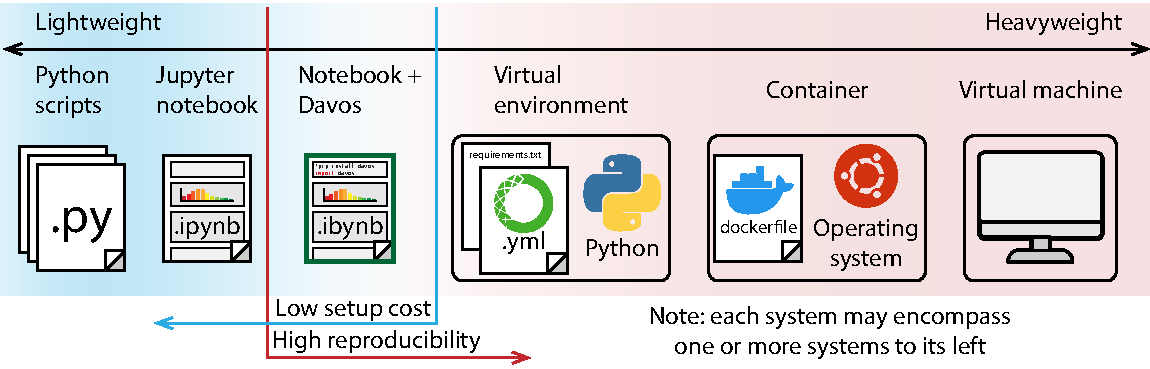
\includegraphics[width=\textwidth]{figs/shareable_code}
\caption{\small \textbf{Systems for sharing code within the Python
    ecosystem.}  From left to right: plain-text \textbf{Python
    scripts} (.py files) provide the
  most basic ``system'' for sharing raw code.  Scripts may reference
  external libraries, but those libraries are not automatically
  installed on other users' systems, nor is any version checking
  performed by default.  \textbf{Jupyter notebooks} (.ipynb files) comprise embedded text,
  executable code, and media (including rendered figures, code output,
  etc.).  When the \textbf{\texttt{davos} library} is imported into a Jupyter
  notebook, the notebook's functionality is extended to automatically
  install the required external libraries (at their correct versions,
  when specified).  \textbf{Virtual environments} install an isolated copy of
  Python and all required dependencies.  This typically requires
  defining a \texttt{requirements.txt} file that lists all
  dependencies (including version numbers) along with an environment
  (.yml) file that specifies how the virtual environment should be
  configured.  \textbf{Containers} provide a means of defining an isolated
  environment that includes a complete operating system (independent
  of the user's operating system), in addition to a virtual
  environment or other configurations needed to provide the necessary
  computing environment.  Containers are typically defined using
  specification files (e.g., a plain-text \texttt{dockerfile}) that
  instruct the virtualization engine regarding how to build the
  virtual environment.  \textbf{Virtual machines} provide a complete
  hardware-level simulation of the computing environment.  In addition
  to simulating specific hardware, virtual machines (typically
  specified using binary images files) must also define operating
  system-level properties of the computing environment.  Systems to
  the left of the blue vertical line entail sharing individual
  files, with no additional installation or configuration needed to
  run the target software.  Systems to the right of the red vertical
  line provide high reproducibility by supporting precise control over
  dependencies and versioning.  Notebooks enhanced using the
  \texttt{davos} library are easily shareable and require minimal
  setup costs, while also facilitating high reproducibility by
  enabling precise control over project dependencies.}
\label{fig:code-sharing}
\end{figure}

To facilitate code sharing, the Python community has developed a broad
set of approaches and tools (Fig.~\ref{fig:code-sharing}).  At one
extreme, simply publishing a set of Python scripts (.py files) may
enable others to use or gain insights into the relevant work.  Because
Python is installed by default on most modern operating systems, for
some projects this may be sufficient.  Another popular approach
entails creating JSON files, called Jupyter
notebooks~\citep{KluyEtal16}, that comprise a mix of text, executable
code, and embedded media.  Notebooks may call or import external
scripts or libraries in order to provide a more compact and readable
experience for users.  Each of these systems (Python scripts and
notebooks) provides a convenient means of sharing code, with the
caveat that they do not specify the computing environment in which the
code is executed.  Therefore the functionality of code shared using
these systems cannot be guaranteed across different computing
environments.

At another extreme, virtual machines~\citep{Gold74, AltiEtal05,
  vmware} provide a hardware-level simulation of the desired system.
Virtual machines are typically isolated from the user's system, such
that installing or running software on a virtual machine does not
impact the user's primary operating system or computing environment.
Containers~\citep[e.g.,][]{Merk14, KurtEtal17} provide a similar
``isolated'' experience.  Although containerized environments do not
specify hardware-level operations, they are typically packaged with a
complete operating system, in addition to a complete copy of Python
and any relevant package dependencies.  Virtual
environments~\citep[e.g.,][]{vanREtal14} also provide a computing
environment that is largely separated from the user's main
environment.  They incorporate a copy of Python and the target
software's dependencies, but virtual environments do not specify or
reproduce an operating system for the runtime environment.  Each of
these systems (virtual machines, containers, and virtual environments)
guarantees (to differing degrees-- at the hardware level, operating
system level, and Python environment level, respectively) that the
relevant code will run similarly for different users.  However, each
of these systems also relies on additional software that can be
resource intensive or burdensome to install or configure.

We designed \texttt{davos} to occupy a ``sweet spot'' between these
extremes.  \texttt{davos} is a notebook-installable package that adds
functionality to the default notebook experience.  Like standard
Jupyter notebooks, \texttt{davos}-enhanced notebooks allows
researchers to include text, executable code, and media within a
single file.  No further setup or installation is required, beyond
what is needed to run standard Jupyter notebooks.  And like virtual
environments \texttt{davos} provides a convenient mechanism for fully
specifying (and installing, as needed) a complete set of Python
dependencies, including package versions.




% ------------------------------------------------ SOFTWARE DESCRIPTION ------------------------------------------------
\section{Software description}
% Describe the software in as much as is necessary to establish a vocabulary needed to explain its impact.


\subsection{Software architecture}
The \texttt{davos} package is structured as two sub-packages: a set of ``core" modules that implement...

% Give a short overview of the overall software architecture; provide a pictorial component overview or similar (if possible). If necessary provide implementation details.


\subsection{Software functionalities}%\label{sec:functionalities}

\subsubsection{The \texttt{smuggle} statement}
Importing \texttt{davos}\comment{in a Jupyter notebook} enables an additional Python keyword: ``\texttt{smuggle}".
The \texttt{smuggle} statement can be used as a drop-in replacement for Python's built-in \texttt{import} statement to load libraries, modules, and other objects into the current namespace.
However, whereas \texttt{import} will fail if the requested package is not installed locally, \texttt{smuggle} statements can handle missing packages on the fly.
If a smuggled package does not exist in the local environment, \texttt{davos} will install it, expose its contents to Python's \texttt{import} machinery, and load it into the namespace for immediate use.


\subsubsection{The onion comment}
For greater control over the behavior of \texttt{smuggle} statements, \texttt{davos} defines an additional construct called the \textit{onion comment}. An onion comment is a special type of inline comment that may be placed on a line containing a \texttt{smuggle} statement to customize how \texttt{davos} searches for the smuggled package locally and, if necessary, how it should be installed. Onion comments follow a simple syntax based on the ``type comment" syntax introduced in PEP 484 \cite{vanREtal14} and are designed to make managing packages via \texttt{davos} intuitive and familiar. To construct an onion comment, simply provide the name of the installer program (e.g., \texttt{pip}) and the same arguments one would use to install the package as desired manually via the command line (see Fig.~\ref{fig:snippet1}).

\begin{figure}[h]
\centering
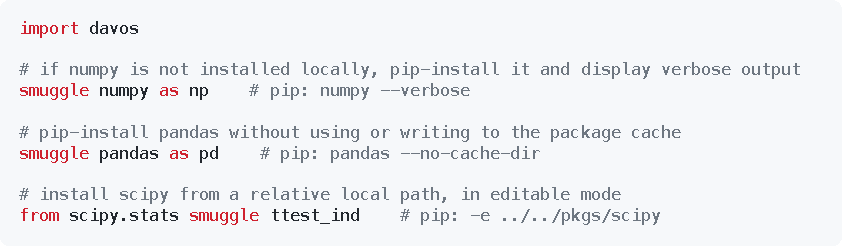
\includegraphics[width=\textwidth]{snippets/snippet1.pdf}
\caption{\small \textbf{FILL THIS IN...}}
\label{fig:snippet1}
\end{figure}



%\definecolor{backgroundgrey}{RGB}{244,246,249}
%\definecolor{commentgrey}{RGB}{91,99,110}
%\definecolor{keywordred}{RGB}{194,11,36}
%
%\lstset{
%    backgroundcolor=\color{backgroundgrey},
%    basicstyle=\footnotesize\fontfamily{qag}\selectfont, %\ttfamily,
%    breaklines=true,
%    commentstyle=\color{commentgrey},
%    language=Python,
%    emph={import, smuggle, from, as},
%    emphstyle=\color{keywordred},
%}
%
%\begin{lstlisting}
%import davos
%
%# if numpy is not installed locally, pip-install it and display verbose output
%smuggle numpy as np    # pip: numpy --verbose
%
%# pip-install pandas without using or writing to the package cache
%smuggle pandas as pd    # pip: pandas --no-cache-dir
%
%# install scipy from a relative local path, in editable mode
%from scipy.stats smuggle ttest_ind # pip: -e ../../pkgs/scipy
%\end{lstlisting}

\subsubsection{The \texttt{davos} config}

\subsubsection{Additional functionality}

% Present the major functionalities of the software.


\subsection{Sample code snippets analysis (optional)}


% ----------------------------------------------- ILLUSTRATIVE EXAMPLES ------------------------------------------------
\section{Illustrative Examples}
% Provide at least one illustrative example to demonstrate the major functions.

% Optional: you may include one explanatory video that will appear next to your article, in the right hand side panel. (Please upload any video as a single supplementary file with your article. Only one MP4 formatted, with 50MB maximum size, video is possible per article. Recommended video dimensions are 640 x 480 at a maximum of 30 frames/second. Prior to submission please test and validate your .mp4 file at $ http://elsevier-apps.sciverse.com/GadgetVideoPodcastPlayerWeb/verification$. This tool will display your video exactly in the same way as it will appear on ScienceDirect.).


% ------------------------------------------------------- IMPACT -------------------------------------------------------
\section{Impact}

Like virtual environments, containers, and virtual machines, the
\texttt{davos} library (when used in conjunction with Jupyter
notebooks) provides a lightweight mechanism for sharing code and
ensuring reproducibility across users and computing environments
(Fig.~\ref{fig:code-sharing}).  Further, \texttt{davos} enables users
to fully specify (and install, as needed) any project dependencies
within the same notebook.  This provides a system whereby executable
code (along with text and media) \textit{and} code for setting up and
configuring the project dependencies, may be combined within a single
notebook file.

We designed \texttt{davos} for use in research applications.  For
example, in many settings \texttt{davos} may be used as a drop-in
replacement for more-difficult-to-set-up virtual environments,
containers, and/or virtual machines.  For researchers, this lowers
barriers to sharing code.  By eliminating most of the setup costs
of reconstructing the original researchers' computing environment,
\texttt{davos} also lowers barriers to entry for members of
the scientific community and the public who seek to \textit{benefit}
from shared code.

Beyond research applications, \texttt{davos} is also useful in
pedagogical settings.  For example, in programming courses,
instructors and students may import the \texttt{davos} library into
their notebooks to provide a simple means of ensuring their code will
run on others' machines.  When combined with online notebook-based
platforms like Google Colaboratory, \texttt{davos} provides a
convenient way to manage dependencies within a notebook, without
requiring any software (beyond a web browser) to be installed on the
students' or instructors' systems.  For the same reasons,
\texttt{davos} also provides an elegant means of sharing ready-to-run
notebook-based demonstrations that install their dependencies
automatically.

Our work also has several more subtle ``advanced'' use cases and
potential impacts.  Whereas Python's built-in \texttt{import}
statement is agnostic to packages' version numbers, \texttt{smuggle}
statements (when combined with onion comments) are version-sensitive.
This enables multiple versions of a single library to be
imported within the same notebook.  This could be useful in cases
where specific features were added or removed from a package across
different versions, or in comparing the performance or functionality
of particular features across different versions of the same package.

A second advanced use case is in providing a proof-of-concept of how
one can add new ``keywords'' to the Python language by leveraging the
error-handling mechanisms.  This could lead to exciting new tools
that, like \texttt{davos}, extend the Python language in useful ways.
We note that our approach to adding the \texttt{smuggle} keyword to
Python when \texttt{davos} is imported into a notebook-based
environment also has the potential to be exploited for more nefarious
purposes.  For example, a malicious user could use a similar approach
(e.g., in a different library) to substantially change a notebook's
functionality by adding new \textit{unexpected} keyword-like objects
(e.g., based around common typos).  This could lead to
difficult-to-predict changes in a notebook's behavior once the
malicious library was imported.  This highlights an important reason
why security-conscious users would be well-served to only make use of
libraries from trusted sources, or whose code is publicly available
for review.

% ---------------------------------------------------- CONCLUSIONS -----------------------------------------------------
\section{Conclusions}
% Set out the conclusion of this original software publication.

The \texttt{davos} library supports reproducible research by providing
a novel lightweight system for sharing notebook-based code.  But
perhaps the most exciting uses of the \texttt{davos} library are those
that we have \textit{not} yet considered or imagined.  We hope that
the Python community will find \texttt{davos} to provide a convenient
means of managing project dependencies to facilitate code sharing.  We
also hope that some of the more advanced applications of our library
might lead to new insights or discoveries.


\section*{Author Contributions}
Conceptualization: PCF and JRM.  Methodology: PCF and JRM.
Implementation: PCF.  Validation: PCF.  Testing: PCF and JRM.
Writing: PCF and JRM.

\section*{Funding}
Our work was supported in part by NSF grant number 2145172 to JRM.
The content is solely the responsibility of the authors and does not necessarily represent the official views of our supporting organizations.


\section*{Declaration of Competing Interest}
We wish to confirm that there are no known conflicts of interest associated with this publication and there has been no significant financial support for this work that could have influenced its outcome.


\section*{Acknowledgements}
We acknowledge useful feedback and discussion from the students of
JRM's \textit{Storytelling with Data} course (Winter, 2022 offering)
who used preliminary versions of our library in several assignments.

%---------------------------------------------------- BIBLIOGRAPHY -----------------------------------------------------
\bibliographystyle{elsarticle-num}
\bibliography{main.bib}

\end{document}

